% !TEX root=./adl.tex

% -----------------------------------------------------------------------
\begin{frame}{Tensor Parallelism --- Overview}

  \emphdef{Tensor Parallelism} (TP) shards individual weight matrices \emph{within} each layer across GPUs~\cite{shoeybi2020megatronlm}.

  \vspace{0.5em}
  \begin{columns}
    \begin{column}{0.48\textwidth}
      \textbf{Core idea:}
      \begin{itemize}
        \item A Transformer layer is dominated by large matrix multiplications $Y = X \cdot W$
        \item Split $W$ into $N$ shards, one per GPU
        \item Each GPU computes with its shard \emph{only} --- partial results are combined via collective communication
        \item Each GPU stores and computes with only $\frac{1}{N}$ of each weight matrix
      \end{itemize}

      \vspace{0.3em}
      \textbf{What is sharded?}
      \begin{itemize}
        \item Weights, gradients, optimizer states $\checkmark$
        \item \textbf{Activations} $\checkmark$ (unlike DP/ZeRO)
      \end{itemize}
    \end{column}
    \begin{column}{0.48\textwidth}
      \textbf{Key difference to Data Parallelism / ZeRO:}
      \begin{itemize}
        \item DP: each GPU has a \emph{full copy} of the model, processes different data
        \item ZeRO: shards parameters but must \emph{gather} full parameters before each computation
        \item TP: each GPU computes with its \emph{shard only} --- no parameter gathering needed!
      \end{itemize}

      \vspace{0.3em}
      \textbf{Communication:}
      \begin{itemize}
        \item Requires AllReduce / AllGather \emph{after each layer} (on the critical path)
        \item Must use fast interconnect (NVLink)
        \item Practical limit: TP degree $\leq$ GPUs per node (typically $\leq 8$)
      \end{itemize}
    \end{column}
  \end{columns}
\end{frame}

% -----------------------------------------------------------------------
\begin{frame}{Linear Layers --- Sharding Potential}

  A Transformer is dominated by linear layers: $Y = X \cdot W$.

  \vspace{0.2em}
  \begin{center}
  \scalebox{0.82}{%
  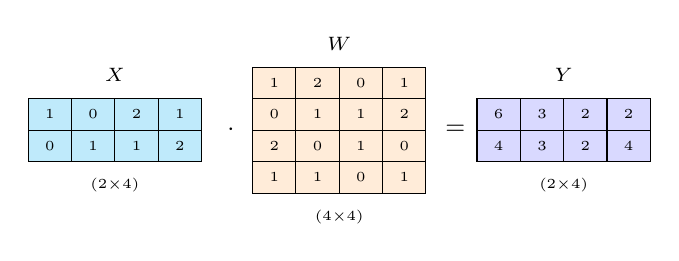
\begin{tikzpicture}[
    cell/.style={draw, minimum width=0.55cm, minimum height=0.4cm, font=\tiny, inner sep=0pt},
    lbl/.style={font=\scriptsize},
  ]
    % X (2x4)
    \node[lbl] at (0.825, 0.7) {$X$};
    \foreach \r/\va/\vb/\vc/\vd in {0/1/0/2/1, 1/0/1/1/2} {
      \node[cell, fill=cyan!25] at (0, 0.2-\r*0.4) {\va};
      \node[cell, fill=cyan!25] at (0.55, 0.2-\r*0.4) {\vb};
      \node[cell, fill=cyan!25] at (1.1, 0.2-\r*0.4) {\vc};
      \node[cell, fill=cyan!25] at (1.65, 0.2-\r*0.4) {\vd};
    }
    \node[lbl] at (0.825, -0.7) {\tiny$(2{\times}4)$};

    % dot
    \node[font=\small] at (2.3, 0) {$\cdot$};

    % W (4x4)
    \node[lbl] at (3.675, 1.1) {$W$};
    \foreach \r/\va/\vb/\vc/\vd in {0/1/2/0/1, 1/0/1/1/2, 2/2/0/1/0, 3/1/1/0/1} {
      \node[cell, fill=orange!15] at (2.85, 0.6-\r*0.4) {\va};
      \node[cell, fill=orange!15] at (3.4, 0.6-\r*0.4) {\vb};
      \node[cell, fill=orange!15] at (3.95, 0.6-\r*0.4) {\vc};
      \node[cell, fill=orange!15] at (4.5, 0.6-\r*0.4) {\vd};
    }
    \node[lbl] at (3.675, -1.1) {\tiny$(4{\times}4)$};

    % equals
    \node[font=\small] at (5.15, 0) {$=$};

    % Y (2x4)
    \node[lbl] at (6.525, 0.7) {$Y$};
    \foreach \r/\va/\vb/\vc/\vd in {0/6/3/2/2, 1/4/3/2/4} {
      \node[cell, fill=blue!15] at (5.7, 0.2-\r*0.4) {\va};
      \node[cell, fill=blue!15] at (6.25, 0.2-\r*0.4) {\vb};
      \node[cell, fill=blue!15] at (6.8, 0.2-\r*0.4) {\vc};
      \node[cell, fill=blue!15] at (7.35, 0.2-\r*0.4) {\vd};
    }
    \node[lbl] at (6.525, -0.7) {\tiny$(2{\times}4)$};
  \end{tikzpicture}}
  \end{center}

  \vspace{0.2em}
  {\small
  \textbf{Problem:} In large models, $W$ has shape $d_\text{model} \times d_\text{model}$
  (e.g.\ $12288 \times 12288$ in GPT-3 $\to$ 600M params per layer).
  Weights, gradients, and optimizer states of a single layer can exceed one GPU's memory.

  \vspace{0.2em}
  \textbf{Solution:} Shard $W$ across $N$ GPUs --- two natural ways to split a matrix:
  }

  \vspace{0.2em}
  \begin{columns}[T]
    \begin{column}{0.45\textwidth}
      \begin{center}
      {\small \textbf{Column split} --- output dim}

      \vspace{0.1em}
      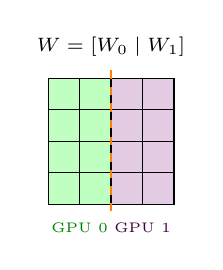
\begin{tikzpicture}[
        cell/.style={minimum width=0.4cm, minimum height=0.4cm, draw, font=\tiny, inner sep=0pt},
        lbl/.style={font=\scriptsize},
      ]
        \foreach \r in {0,...,3} {
          \foreach \c [evaluate=\c as \clr using {ifthenelse(\c<2,"green!25","violet!20")}] in {0,...,3} {
            \node[cell, fill=\clr] at (\c*0.4, -\r*0.4) {};
          }
        }
        \draw[thick, dashed, orange] (0.6, 0.3) -- (0.6, -1.5);
        \node[lbl] at (0.6, 0.6) {$W = [W_0 \mid W_1]$};
        \node[lbl, green!50!black] at (0.2, -1.7) {\tiny GPU 0};
        \node[lbl, violet!50!black] at (1.0, -1.7) {\tiny GPU 1};
      \end{tikzpicture}

      {\footnotesize $X [W_0 \mid W_1] = [XW_0 \mid XW_1]$}
      \end{center}
    \end{column}
    \begin{column}{0.45\textwidth}
      \begin{center}
      {\small \textbf{Row split} --- input dim}

      \vspace{0.1em}
      \begin{tikzpicture}[
        cell/.style={minimum width=0.4cm, minimum height=0.4cm, draw, font=\tiny, inner sep=0pt},
        lbl/.style={font=\scriptsize},
      ]
        \foreach \r [evaluate=\r as \rlr using {ifthenelse(\r<2,"green!25","violet!20")}] in {0,...,3} {
          \foreach \c in {0,...,3} {
            \node[cell, fill=\rlr] at (\c*0.4, -\r*0.4) {};
          }
        }
        \draw[thick, dashed, orange] (-0.3, -0.6) -- (1.5, -0.6);
        \node[lbl] at (0.6, 0.6) {$W = \left[\begin{smallmatrix} W_0 \\ W_1 \end{smallmatrix}\right]$};
        \node[lbl, green!50!black, anchor=west] at (1.5, -0.2) {\tiny GPU 0};
        \node[lbl, violet!50!black, anchor=west] at (1.5, -1.0) {\tiny GPU 1};
      \end{tikzpicture}

      {\footnotesize $[X_0 \mid X_1]\!\left[\begin{smallmatrix} W_0 \\ W_1 \end{smallmatrix}\right] = X_0 W_0 {+} X_1 W_1$}
      \end{center}
    \end{column}
  \end{columns}
\end{frame}

% -----------------------------------------------------------------------
\begin{frame}{Column-Parallel Linear Layer}

  Split the weight matrix $W$ by \textbf{columns}, keep the full input $X$ on every GPU.

  \vspace{0.2em}
  \begin{center}
  \scalebox{0.82}{%
  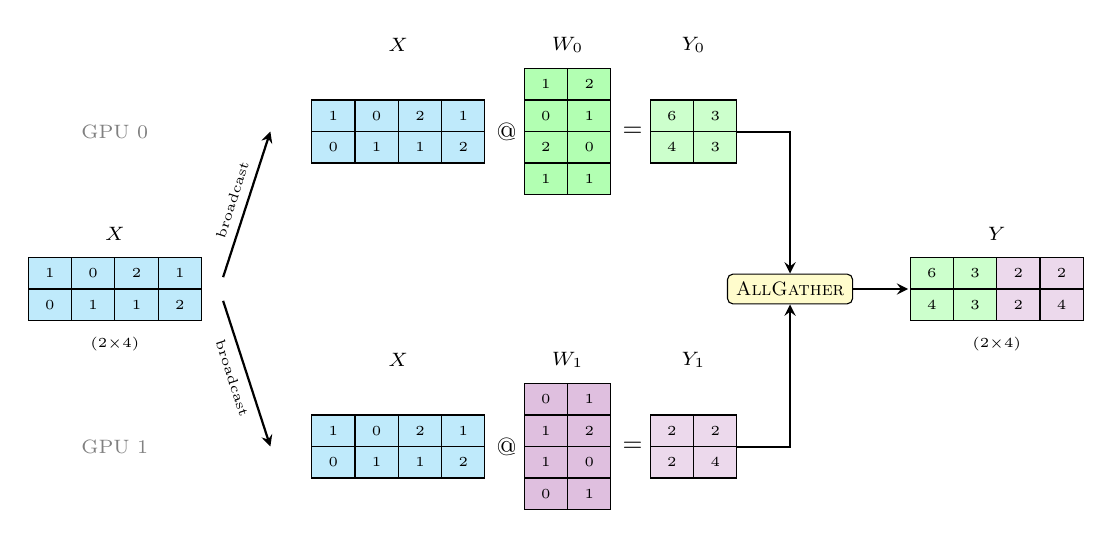
\begin{tikzpicture}[
    cell/.style={draw, minimum width=0.55cm, minimum height=0.4cm, font=\tiny, inner sep=0pt},
    arr/.style={->, thick, >=stealth},
    op/.style={font=\scriptsize, fill=yellow!20, draw, rounded corners=2pt, inner sep=3pt},
    lbl/.style={font=\scriptsize},
    gpulbl/.style={font=\scriptsize, gray},
    ds/.style={draw, dashed, rounded corners=3pt, cyan!50, inner sep=4pt},
  ]
    % Vertical centers: symmetric around source X at y=0
    \def\gtop{2.0}   % GPU 0 center
    \def\gbot{-2.0}  % GPU 1 center

    % === Source X (2x4, left) ===
    \node[lbl] at (-2.775, 0.7) {$X$};
    \foreach \r/\va/\vb/\vc/\vd in {0/1/0/2/1, 1/0/1/1/2} {
      \node[cell, fill=cyan!25] at (-3.6, 0.2-\r*0.4) {\va};
      \node[cell, fill=cyan!25] at (-3.05, 0.2-\r*0.4) {\vb};
      \node[cell, fill=cyan!25] at (-2.5, 0.2-\r*0.4) {\vc};
      \node[cell, fill=cyan!25] at (-1.95, 0.2-\r*0.4) {\vd};
    }
    \node[lbl] at (-2.775, -0.7) {\tiny$(2{\times}4)$};

    % Broadcast arrows
    \draw[arr] (-1.4, 0.15) -- node[above, font=\tiny, sloped] {broadcast} (-0.8, \gtop);
    \draw[arr] (-1.4,-0.15) -- node[below, font=\tiny, sloped] {broadcast} (-0.8, \gbot);

    % GPU labels (above/below source X, at GPU section heights)
    \node[gpulbl] at (-2.775, \gtop) {GPU 0};
    \node[gpulbl] at (-2.775, \gbot) {GPU 1};

    % === GPU 0 ===

    % X copy (2x4)
    \foreach \r/\va/\vb/\vc/\vd in {0/1/0/2/1, 1/0/1/1/2} {
      \node[cell, fill=cyan!25] at (0, \gtop+0.2-\r*0.4) {\va};
      \node[cell, fill=cyan!25] at (0.55, \gtop+0.2-\r*0.4) {\vb};
      \node[cell, fill=cyan!25] at (1.1, \gtop+0.2-\r*0.4) {\vc};
      \node[cell, fill=cyan!25] at (1.65, \gtop+0.2-\r*0.4) {\vd};
    }
    \node[lbl] at (0.825, \gtop+1.1) {$X$};

    % @
    \node[font=\small] at (2.2, \gtop) {$@$};

    % W_0 (4x2, first 2 columns of W)
    \node[lbl] at (2.975, \gtop+1.1) {$W_0$};
    \foreach \r/\va/\vb in {0/1/2, 1/0/1, 2/2/0, 3/1/1} {
      \node[cell, fill=green!30] at (2.7, \gtop+0.6-\r*0.4) {\va};
      \node[cell, fill=green!30] at (3.25, \gtop+0.6-\r*0.4) {\vb};
    }

    % =
    \node[font=\small] at (3.8, \gtop) {$=$};

    % Y_0 (2x2)
    \node[lbl] at (4.575, \gtop+1.1) {$Y_0$};
    \foreach \r/\va/\vb in {0/6/3, 1/4/3} {
      \node[cell, fill=green!20] (y0\r a) at (4.3, \gtop+0.2-\r*0.4) {\va};
      \node[cell, fill=green!20] (y0\r b) at (4.85, \gtop+0.2-\r*0.4) {\vb};
    }

    % === GPU 1 ===

    % X copy (2x4)
    \foreach \r/\va/\vb/\vc/\vd in {0/1/0/2/1, 1/0/1/1/2} {
      \node[cell, fill=cyan!25] at (0, \gbot+0.2-\r*0.4) {\va};
      \node[cell, fill=cyan!25] at (0.55, \gbot+0.2-\r*0.4) {\vb};
      \node[cell, fill=cyan!25] at (1.1, \gbot+0.2-\r*0.4) {\vc};
      \node[cell, fill=cyan!25] at (1.65, \gbot+0.2-\r*0.4) {\vd};
    }
    \node[lbl] at (0.825, \gbot+1.1) {$X$};

    % @
    \node[font=\small] at (2.2, \gbot) {$@$};

    % W_1 (4x2, last 2 columns of W)
    \node[lbl] at (2.975, \gbot+1.1) {$W_1$};
    \foreach \r/\va/\vb in {0/0/1, 1/1/2, 2/1/0, 3/0/1} {
      \node[cell, fill=violet!25] at (2.7, \gbot+0.6-\r*0.4) {\va};
      \node[cell, fill=violet!25] at (3.25, \gbot+0.6-\r*0.4) {\vb};
    }

    % =
    \node[font=\small] at (3.8, \gbot) {$=$};

    % Y_1 (2x2)
    \node[lbl] at (4.575, \gbot+1.1) {$Y_1$};
    \foreach \r/\va/\vb in {0/2/2, 1/2/4} {
      \node[cell, fill=violet!15] (y1\r a) at (4.3, \gbot+0.2-\r*0.4) {\va};
      \node[cell, fill=violet!15] (y1\r b) at (4.85, \gbot+0.2-\r*0.4) {\vb};
    }

    % === AllGather ===
    \node[op] (ag) at (5.8, 0) {\textsc{AllGather}};
    \draw[arr] (y00b.south east) -| (ag.north);
    \draw[arr] (y10b.south east) -| (ag.south);

    % === Final Y (2x4) ===
    \node[lbl] at (8.425, 0.7) {$Y$};
    \foreach \r/\va/\vb/\vc/\vd in {0/6/3/2/2, 1/4/3/2/4} {
      \node[cell, fill=green!20] at (7.6, 0.2-\r*0.4) {\va};
      \node[cell, fill=green!20] at (8.15, 0.2-\r*0.4) {\vb};
      \node[cell, fill=violet!15] at (8.7, 0.2-\r*0.4) {\vc};
      \node[cell, fill=violet!15] at (9.25, 0.2-\r*0.4) {\vd};
    }
    \node[lbl] at (8.425, -0.7) {\tiny$(2{\times}4)$};

    \draw[arr] (ag.east) -- (7.3, 0);
  \end{tikzpicture}}
  \end{center}

  \begin{columns}
    \begin{column}{0.48\textwidth}
      \textbf{Forward:}
      \begin{enumerate}
        \item Broadcast $X$ to all GPUs (or it is already replicated)
        \item Each GPU $i$: $Y_i = X \cdot W_i$
        \item \textsc{AllGather} to get $Y = [Y_0 \mid \cdots \mid Y_{N-1}]$
      \end{enumerate}
    \end{column}
    \begin{column}{0.48\textwidth}
      \textbf{Properties:}
      \begin{itemize}
        \item Output $Y$ is split along the \emph{output feature} dimension
        \item Each GPU stores only $\frac{1}{N}$ of $W$
        \item Useful when the next operation can work on the split output (e.g.\ GeLU)
      \end{itemize}
    \end{column}
  \end{columns}
\end{frame}

% -----------------------------------------------------------------------
\begin{frame}{Row-Parallel Linear Layer}

  Split the weight matrix $W$ by \textbf{rows} and the input $X$ by \textbf{columns}.

  \vspace{0.3em}
  \begin{center}
  \scalebox{0.82}{%
  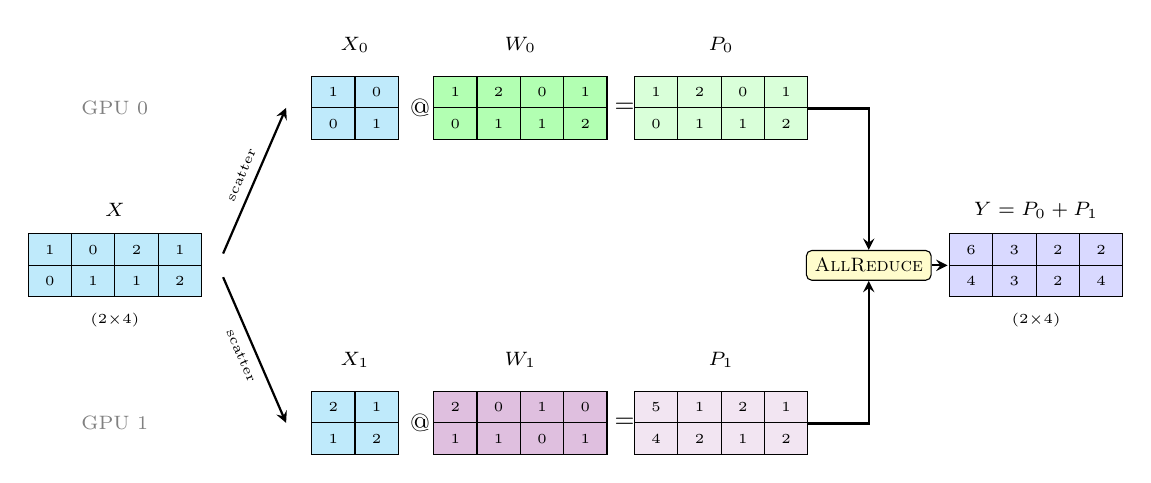
\begin{tikzpicture}[
    cell/.style={draw, minimum width=0.55cm, minimum height=0.4cm, font=\tiny, inner sep=0pt},
    arr/.style={->, thick, >=stealth},
    op/.style={font=\scriptsize, fill=yellow!20, draw, rounded corners=2pt, inner sep=3pt},
    lbl/.style={font=\scriptsize},
    gpulbl/.style={font=\scriptsize, gray},
  ]
    % Vertical centers: symmetric around y=0
    \def\gtop{2.0}   % GPU 0 center
    \def\gbot{-2.0}  % GPU 1 center

    % === Source X (2x4, left) ===
    \node[lbl] at (-2.775, 0.7) {$X$};
    \foreach \r/\va/\vb/\vc/\vd in {0/1/0/2/1, 1/0/1/1/2} {
      \node[cell, fill=cyan!25] at (-3.6, 0.2-\r*0.4) {\va};
      \node[cell, fill=cyan!25] at (-3.05, 0.2-\r*0.4) {\vb};
      \node[cell, fill=cyan!25] at (-2.5, 0.2-\r*0.4) {\vc};
      \node[cell, fill=cyan!25] at (-1.95, 0.2-\r*0.4) {\vd};
    }
    \node[lbl] at (-2.775, -0.7) {\tiny$(2{\times}4)$};

    % Scatter arrows
    \draw[arr] (-1.4, 0.15) -- node[above, font=\tiny, sloped] {scatter} (-0.6, \gtop);
    \draw[arr] (-1.4,-0.15) -- node[below, font=\tiny, sloped] {scatter} (-0.6, \gbot);

    % GPU labels (above/below source X)
    \node[gpulbl] at (-2.775, \gtop) {GPU 0};
    \node[gpulbl] at (-2.775, \gbot) {GPU 1};

    % === GPU 0 ===

    % X_0 (2x2) - first 2 columns of X
    \node[lbl] at (0.275, \gtop+0.8) {$X_0$};
    \foreach \r/\va/\vb in {0/1/0, 1/0/1} {
      \node[cell, fill=cyan!25] at (0, \gtop+0.2-\r*0.4) {\va};
      \node[cell, fill=cyan!25] at (0.55, \gtop+0.2-\r*0.4) {\vb};
    }

    % @
    \node[font=\small] at (1.1, \gtop) {$@$};

    % W_0 (2x4) - first 2 rows of W
    \node[lbl] at (2.375, \gtop+0.8) {$W_0$};
    \foreach \r/\va/\vb/\vc/\vd in {0/1/2/0/1, 1/0/1/1/2} {
      \node[cell, fill=green!30] at (1.55, \gtop+0.2-\r*0.4) {\va};
      \node[cell, fill=green!30] at (2.1, \gtop+0.2-\r*0.4) {\vb};
      \node[cell, fill=green!30] at (2.65, \gtop+0.2-\r*0.4) {\vc};
      \node[cell, fill=green!30] at (3.2, \gtop+0.2-\r*0.4) {\vd};
    }

    % =
    \node[font=\small] at (3.7, \gtop) {$=$};

    % P_0 (2x4) - partial result
    \node[lbl] at (4.925, \gtop+0.8) {$P_0$};
    \foreach \r/\va/\vb/\vc/\vd in {0/1/2/0/1, 1/0/1/1/2} {
      \node[cell, fill=green!15] (p0\r a) at (4.1, \gtop+0.2-\r*0.4) {\va};
      \node[cell, fill=green!15] (p0\r b) at (4.65, \gtop+0.2-\r*0.4) {\vb};
      \node[cell, fill=green!15] (p0\r c) at (5.2, \gtop+0.2-\r*0.4) {\vc};
      \node[cell, fill=green!15] (p0\r d) at (5.75, \gtop+0.2-\r*0.4) {\vd};
    }

    % === GPU 1 ===

    % X_1 (2x2) - last 2 columns of X
    \node[lbl] at (0.275, \gbot+0.8) {$X_1$};
    \foreach \r/\va/\vb in {0/2/1, 1/1/2} {
      \node[cell, fill=cyan!25] at (0, \gbot+0.2-\r*0.4) {\va};
      \node[cell, fill=cyan!25] at (0.55, \gbot+0.2-\r*0.4) {\vb};
    }

    % @
    \node[font=\small] at (1.1, \gbot) {$@$};

    % W_1 (2x4) - last 2 rows of W
    \node[lbl] at (2.375, \gbot+0.8) {$W_1$};
    \foreach \r/\va/\vb/\vc/\vd in {0/2/0/1/0, 1/1/1/0/1} {
      \node[cell, fill=violet!25] at (1.55, \gbot+0.2-\r*0.4) {\va};
      \node[cell, fill=violet!25] at (2.1, \gbot+0.2-\r*0.4) {\vb};
      \node[cell, fill=violet!25] at (2.65, \gbot+0.2-\r*0.4) {\vc};
      \node[cell, fill=violet!25] at (3.2, \gbot+0.2-\r*0.4) {\vd};
    }

    % =
    \node[font=\small] at (3.7, \gbot) {$=$};

    % P_1 (2x4) - partial result
    \node[lbl] at (4.925, \gbot+0.8) {$P_1$};
    \foreach \r/\va/\vb/\vc/\vd in {0/5/1/2/1, 1/4/2/1/2} {
      \node[cell, fill=violet!10] (p1\r a) at (4.1, \gbot+0.2-\r*0.4) {\va};
      \node[cell, fill=violet!10] (p1\r b) at (4.65, \gbot+0.2-\r*0.4) {\vb};
      \node[cell, fill=violet!10] (p1\r c) at (5.2, \gbot+0.2-\r*0.4) {\vc};
      \node[cell, fill=violet!10] (p1\r d) at (5.75, \gbot+0.2-\r*0.4) {\vd};
    }

    % === AllReduce ===
    \node[op] (ar) at (6.8, 0) {\textsc{AllReduce}};
    \draw[arr] (p00d.south east) -| (ar.north);
    \draw[arr] (p10d.south east) -| (ar.south);

    % === Final Y (2x4) - replicated on all GPUs ===
    \node[lbl] at (8.925, 0.7) {$Y = P_0 + P_1$};
    \foreach \r/\va/\vb/\vc/\vd in {0/6/3/2/2, 1/4/3/2/4} {
      \node[cell, fill=blue!15] at (8.1, 0.2-\r*0.4) {\va};
      \node[cell, fill=blue!15] at (8.65, 0.2-\r*0.4) {\vb};
      \node[cell, fill=blue!15] at (9.2, 0.2-\r*0.4) {\vc};
      \node[cell, fill=blue!15] at (9.75, 0.2-\r*0.4) {\vd};
    }
    \node[lbl] at (8.925, -0.7) {\tiny$(2{\times}4)$};

    \draw[arr] (ar.east) -- (7.8, 0);
  \end{tikzpicture}}
  \end{center}

  \vspace{0.2em}
  \begin{columns}
    \begin{column}{0.48\textwidth}
      \textbf{Forward:}
      \begin{enumerate}
        \item Scatter input: GPU $i$ gets $X_i$ (split along feature dim)
        \item Each GPU: partial result $P_i = X_i \cdot W_i$
        \item \textsc{AllReduce} (sum) to get $Y = \sum_i P_i$
      \end{enumerate}
    \end{column}
    \begin{column}{0.48\textwidth}
      \textbf{Properties:}
      \begin{itemize}
        \item Output $Y$ is \emph{replicated} on all GPUs
        \item Complementary to column-parallel: the split output of a column-parallel layer can directly serve as the split input here
      \end{itemize}
    \end{column}
  \end{columns}
\end{frame}

% -----------------------------------------------------------------------
\begin{frame}{TP in the Transformer: MLP Block}

  Key insight: pair \textbf{column-parallel $\to$ row-parallel} to minimize communication~\cite{shoeybi2020megatronlm}.

  \vspace{0.2em}
  \begin{center}
  \scalebox{0.72}{%
  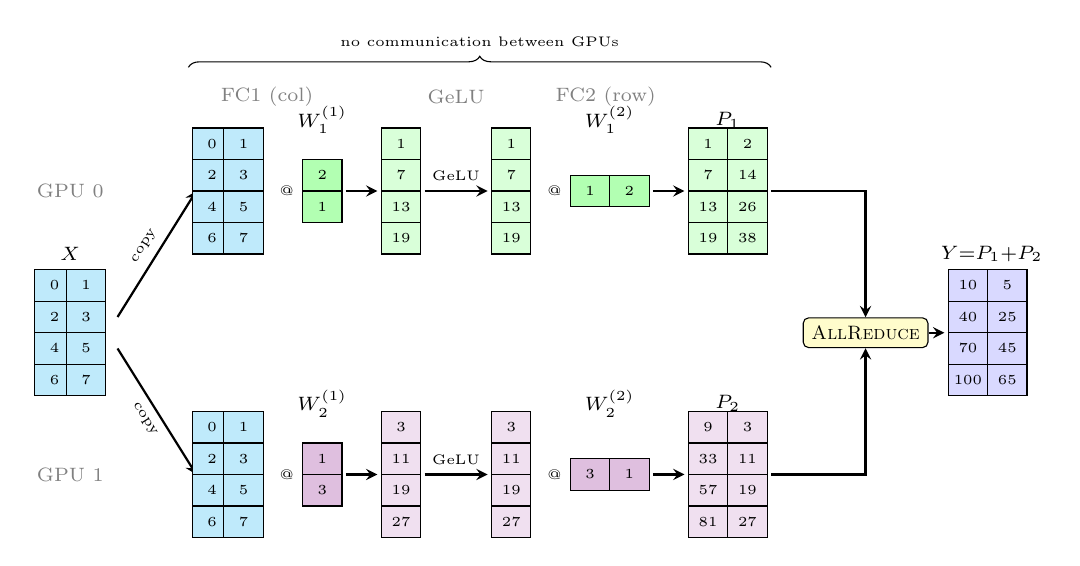
\begin{tikzpicture}[
    cell/.style={draw, minimum width=0.5cm, minimum height=0.4cm, font=\tiny, inner sep=0pt},
    arr/.style={->, thick, >=stealth},
    op/.style={font=\scriptsize, fill=yellow!20, draw, rounded corners=2pt, inner sep=3pt},
    lbl/.style={font=\scriptsize},
    gpulbl/.style={font=\scriptsize, gray},
    stagelbl/.style={font=\scriptsize, gray},
  ]
    \def\gtop{1.8}
    \def\gbot{-1.8}
    \def\cs{0.4}  % cell spacing = cell height

    % === Source X (4x2) ===
    \node[lbl] at (0.2, 1.0) {$X$};
    \foreach \r/\va/\vb in {0/0/1, 1/2/3, 2/4/5, 3/6/7} {
      \node[cell, fill=cyan!25] at (0, 0.6-\r*\cs) {\va};
      \node[cell, fill=cyan!25] at (\cs, 0.6-\r*\cs) {\vb};
    }

    % Broadcast arrows
    \draw[arr] (0.8, 0.2) -- node[above, font=\tiny, sloped] {copy} (1.8, \gtop);
    \draw[arr] (0.8,-0.2) -- node[below, font=\tiny, sloped] {copy} (1.8, \gbot);

    % GPU labels (above/below source X)
    \node[gpulbl] at (0.2, \gtop) {GPU 0};
    \node[gpulbl] at (0.2, \gbot) {GPU 1};

    % Stage labels (centered above corresponding elements)
    \node[stagelbl] at (2.7, \gtop+1.2) {FC1 (col)};
    \node[stagelbl] at (5.1, \gtop+1.2) {GeLU};
    \node[stagelbl] at (7.0, \gtop+1.2) {FC2 (row)};

    % ================================================================
    % GPU 0: X @ W_1^(1) = H_1, GeLU(H_1) = H_1', H_1' @ W_1^(2) = P_1
    % ================================================================

    % X copy (4x2)
    \foreach \r/\va/\vb in {0/0/1, 1/2/3, 2/4/5, 3/6/7} {
      \node[cell, fill=cyan!25] at (2.0, \gtop+0.6-\r*\cs) {\va};
      \node[cell, fill=cyan!25] at (2.0+\cs, \gtop+0.6-\r*\cs) {\vb};
    }

    \node[font=\tiny] at (2.95, \gtop) {$@$};

    % W_1^(1) (2x1)
    \node[lbl] at (3.4, \gtop+0.9) {$W_1^{(1)}$};
    \node[cell, fill=green!30] at (3.4, \gtop+0.2) {2};
    \node[cell, fill=green!30] at (3.4, \gtop-0.2) {1};

    \draw[arr] (3.7, \gtop) -- (4.1, \gtop);

    % H_1 (4x1)
    \node[cell, fill=green!15] at (4.4, \gtop+0.6) {1};
    \node[cell, fill=green!15] at (4.4, \gtop+0.2) {7};
    \node[cell, fill=green!15] at (4.4, \gtop-0.2) {13};
    \node[cell, fill=green!15] at (4.4, \gtop-0.6) {19};

    \draw[arr] (4.7, \gtop) -- node[above, font=\tiny] {GeLU} (5.5, \gtop);

    % H_1' (4x1, GeLU ≈ identity for positive)
    \node[cell, fill=green!15] at (5.8, \gtop+0.6) {1};
    \node[cell, fill=green!15] at (5.8, \gtop+0.2) {7};
    \node[cell, fill=green!15] at (5.8, \gtop-0.2) {13};
    \node[cell, fill=green!15] at (5.8, \gtop-0.6) {19};

    \node[font=\tiny] at (6.35, \gtop) {$@$};

    % W_1^(2) (1x2)
    \node[lbl] at (7.05, \gtop+0.9) {$W_1^{(2)}$};
    \node[cell, fill=green!30] at (6.8, \gtop) {1};
    \node[cell, fill=green!30] at (7.3, \gtop) {2};

    \draw[arr] (7.6, \gtop) -- (8.0, \gtop);

    % P_1 (4x2)
    \node[lbl] at (8.55, \gtop+0.9) {$P_1$};
    \node[cell, fill=green!15] at (8.3, \gtop+0.6) {1};
    \node[cell, fill=green!15] at (8.8, \gtop+0.6) {2};
    \node[cell, fill=green!15] at (8.3, \gtop+0.2) {7};
    \node[cell, fill=green!15] at (8.8, \gtop+0.2) {14};
    \node[cell, fill=green!15] at (8.3, \gtop-0.2) {13};
    \node[cell, fill=green!15] at (8.8, \gtop-0.2) {26};
    \node[cell, fill=green!15] (p10b) at (8.3, \gtop-0.6) {19};
    \node[cell, fill=green!15] at (8.8, \gtop-0.6) {38};

    % ================================================================
    % GPU 1: X @ W_2^(1) = H_2, GeLU(H_2) = H_2', H_2' @ W_2^(2) = P_2
    % ================================================================

    % X copy (4x2)
    \foreach \r/\va/\vb in {0/0/1, 1/2/3, 2/4/5, 3/6/7} {
      \node[cell, fill=cyan!25] at (2.0, \gbot+0.6-\r*\cs) {\va};
      \node[cell, fill=cyan!25] at (2.0+\cs, \gbot+0.6-\r*\cs) {\vb};
    }

    \node[font=\tiny] at (2.95, \gbot) {$@$};

    % W_2^(1) (2x1)
    \node[lbl] at (3.4, \gbot+0.9) {$W_2^{(1)}$};
    \node[cell, fill=violet!25] at (3.4, \gbot+0.2) {1};
    \node[cell, fill=violet!25] at (3.4, \gbot-0.2) {3};

    \draw[arr] (3.7, \gbot) -- (4.1, \gbot);

    % H_2 (4x1)
    \node[cell, fill=violet!12] at (4.4, \gbot+0.6) {3};
    \node[cell, fill=violet!12] at (4.4, \gbot+0.2) {11};
    \node[cell, fill=violet!12] at (4.4, \gbot-0.2) {19};
    \node[cell, fill=violet!12] at (4.4, \gbot-0.6) {27};

    \draw[arr] (4.7, \gbot) -- node[above, font=\tiny] {GeLU} (5.5, \gbot);

    % H_2' (4x1)
    \node[cell, fill=violet!12] at (5.8, \gbot+0.6) {3};
    \node[cell, fill=violet!12] at (5.8, \gbot+0.2) {11};
    \node[cell, fill=violet!12] at (5.8, \gbot-0.2) {19};
    \node[cell, fill=violet!12] at (5.8, \gbot-0.6) {27};

    \node[font=\tiny] at (6.35, \gbot) {$@$};

    % W_2^(2) (1x2)
    \node[lbl] at (7.05, \gbot+0.9) {$W_2^{(2)}$};
    \node[cell, fill=violet!25] at (6.8, \gbot) {3};
    \node[cell, fill=violet!25] at (7.3, \gbot) {1};

    \draw[arr] (7.6, \gbot) -- (8.0, \gbot);

    % P_2 (4x2)
    \node[lbl] at (8.55, \gbot+0.9) {$P_2$};
    \node[cell, fill=violet!12] (p20a) at (8.3, \gbot+0.6) {9};
    \node[cell, fill=violet!12] at (8.8, \gbot+0.6) {3};
    \node[cell, fill=violet!12] at (8.3, \gbot+0.2) {33};
    \node[cell, fill=violet!12] at (8.8, \gbot+0.2) {11};
    \node[cell, fill=violet!12] at (8.3, \gbot-0.2) {57};
    \node[cell, fill=violet!12] at (8.8, \gbot-0.2) {19};
    \node[cell, fill=violet!12] (p20b) at (8.3, \gbot-0.6) {81};
    \node[cell, fill=violet!12] at (8.8, \gbot-0.6) {27};

    % === AllReduce ===
    \node[op] (ar) at (10.3, 0) {\textsc{AllReduce}};
    \draw[arr] (9.1, \gtop) -| (ar.north);
    \draw[arr] (9.1, \gbot) -| (ar.south);

    % === Final Y (4x2) ===
    \node[lbl] at (11.9, 1.0) {$Y{=}P_1{+}P_2$};
    \node[cell, fill=blue!15] at (11.6, 0.6) {10};
    \node[cell, fill=blue!15] at (12.1, 0.6) {5};
    \node[cell, fill=blue!15] at (11.6, 0.2) {40};
    \node[cell, fill=blue!15] at (12.1, 0.2) {25};
    \node[cell, fill=blue!15] at (11.6,-0.2) {70};
    \node[cell, fill=blue!15] at (12.1,-0.2) {45};
    \node[cell, fill=blue!15] at (11.6,-0.6) {100};
    \node[cell, fill=blue!15] at (12.1,-0.6) {65};

    \draw[arr] (ar.east) -- (11.3, 0);

    % No-comm brace
    \draw[decorate, decoration={brace, amplitude=4pt, raise=2pt}]
      (1.7, \gtop+1.5) -- (9.1, \gtop+1.5)
      node[midway, above=6pt, font=\tiny] {no communication between GPUs};
  \end{tikzpicture}}
  \end{center}

  \vspace{0.1em}
  \begin{itemize}\small
    \item \textbf{FC1} (column-parallel): $X$ replicated, each GPU computes with its column shard of $W^{(1)}$
    \item \textbf{GeLU}: element-wise, applied independently on each shard (no communication)
    \item \textbf{FC2} (row-parallel): split GeLU output feeds directly as split input $\to$ partial sums $\to$ AllReduce
    \item Only \textbf{one AllReduce} per MLP block (column$\to$row pairing avoids extra communication)
  \end{itemize}
\end{frame}

% -----------------------------------------------------------------------
\begin{frame}{TP in the Transformer: Attention Block}

  Same column$\to$row pattern: QKV projections (col-parallel) $\to$ attention per head $\to$ output proj (row-parallel).

  \vspace{0.2em}
  \begin{center}
  \scalebox{0.72}{%
  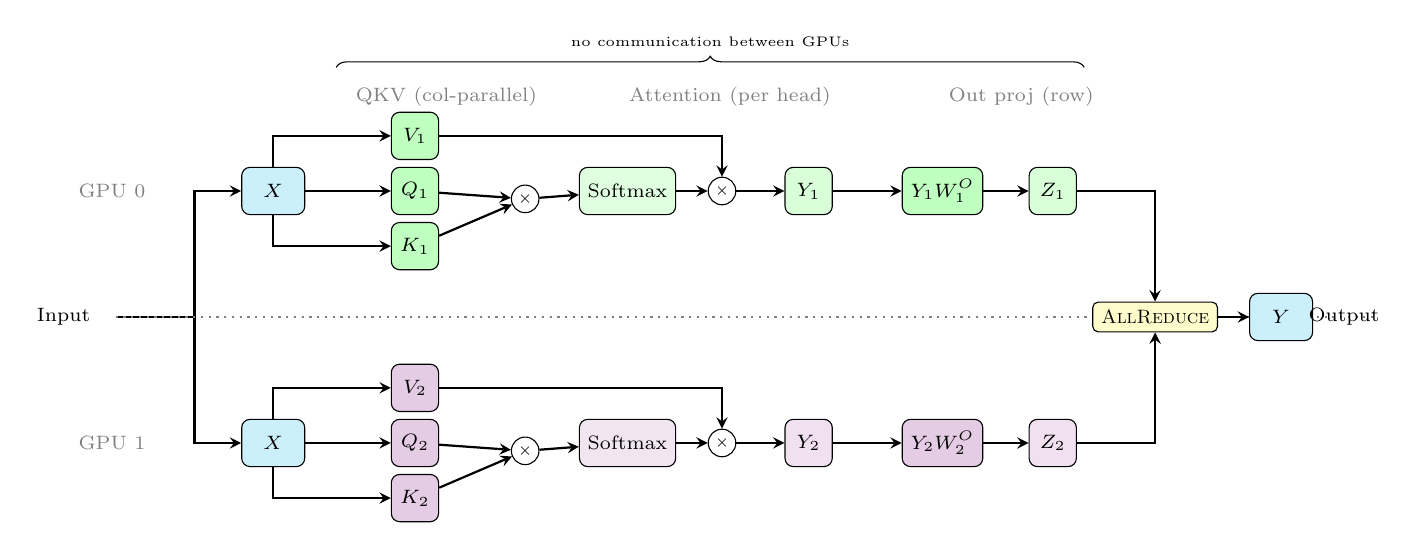
\begin{tikzpicture}[
    block/.style={draw, rounded corners=3pt, minimum height=0.6cm, font=\scriptsize, inner sep=3pt},
    arr/.style={->, thick, >=stealth},
    op/.style={font=\scriptsize, fill=yellow!20, draw, rounded corners=2pt, inner sep=3pt},
    mul/.style={draw, circle, font=\tiny, inner sep=1pt, minimum size=0.35cm},
    lbl/.style={font=\scriptsize},
    gpulbl/.style={font=\scriptsize, gray},
    stagelbl/.style={font=\scriptsize, gray},
  ]
    \def\gtop{1.6}
    \def\gbot{-1.6}

    % === Input X ===
    \node[block, fill=cyan!20, minimum width=0.8cm] (x0) at (0, \gtop) {$X$};
    \node[block, fill=cyan!20, minimum width=0.8cm] (x1) at (0, \gbot) {$X$};
    \node[lbl, left] at (-2.2, 0) {Input};

    \draw[thick] (-2.0, 0) -- (-1.0, 0);
    \draw[arr] (-1.0, 0) |- (x0.west);
    \draw[arr] (-1.0, 0) |- (x1.west);

    % GPU labels
    \node[gpulbl, anchor=east] at (-1.5, \gtop) {GPU 0};
    \node[gpulbl, anchor=east] at (-1.5, \gbot) {GPU 1};

    % Dotted separator
    \draw[dotted, thick, gray] (-2.0, 0) -- (14.0, 0);

    % Stage labels
    \node[stagelbl] at (2.2, \gtop+1.2) {QKV (col-parallel)};
    \node[stagelbl] at (5.8, \gtop+1.2) {Attention (per head)};
    \node[stagelbl] at (9.5, \gtop+1.2) {Out proj (row)};

    % ================================================================
    % GPU 0
    % ================================================================

    % Q1, K1, V1 projections
    \node[block, fill=green!25, minimum width=0.6cm] (q1) at (1.8, \gtop) {$Q_1$};
    \node[block, fill=green!25, minimum width=0.6cm] (k1) at (1.8, \gtop-0.7) {$K_1$};
    \node[block, fill=green!25, minimum width=0.6cm] (v1) at (1.8, \gtop+0.7) {$V_1$};

    \draw[arr] (x0) -- (q1);
    \draw[arr] (x0) |- (k1);
    \draw[arr] (x0) |- (v1);

    % Q1 x K1^T
    \node[mul] (qk1) at (3.2, \gtop-0.1) {$\times$};
    \draw[arr] (q1) -- (qk1);
    \draw[arr] (k1) -- (qk1);

    % Softmax + Dropout
    \node[block, fill=green!12, minimum width=0.9cm] (sm1) at (4.5, \gtop) {Softmax};
    \draw[arr] (qk1) -- (sm1);

    % x V1
    \node[mul] (av1) at (5.7, \gtop) {$\times$};
    \draw[arr] (sm1) -- (av1);
    \draw[arr] (v1.east) -- (5.7, \gtop+0.7) -- (av1.north);

    % Y1 (attention output per head)
    \node[block, fill=green!15, minimum width=0.6cm] (y1) at (6.8, \gtop) {$Y_1$};
    \draw[arr] (av1) -- (y1);

    % Output projection (row-parallel): Y1 @ W_O1
    \node[block, fill=green!25, minimum width=0.9cm] (wo1) at (8.5, \gtop) {$Y_1 W_1^O$};
    \draw[arr] (y1) -- (wo1);

    % Z1 (partial result)
    \node[block, fill=green!15, minimum width=0.6cm] (z1) at (9.9, \gtop) {$Z_1$};
    \draw[arr] (wo1) -- (z1);

    % ================================================================
    % GPU 1
    % ================================================================

    % Q2, K2, V2 projections
    \node[block, fill=violet!20, minimum width=0.6cm] (q2) at (1.8, \gbot) {$Q_2$};
    \node[block, fill=violet!20, minimum width=0.6cm] (k2) at (1.8, \gbot-0.7) {$K_2$};
    \node[block, fill=violet!20, minimum width=0.6cm] (v2) at (1.8, \gbot+0.7) {$V_2$};

    \draw[arr] (x1) -- (q2);
    \draw[arr] (x1) |- (k2);
    \draw[arr] (x1) |- (v2);

    % Q2 x K2^T
    \node[mul] (qk2) at (3.2, \gbot-0.1) {$\times$};
    \draw[arr] (q2) -- (qk2);
    \draw[arr] (k2) -- (qk2);

    % Softmax
    \node[block, fill=violet!10, minimum width=0.9cm] (sm2) at (4.5, \gbot) {Softmax};
    \draw[arr] (qk2) -- (sm2);

    % x V2
    \node[mul] (av2) at (5.7, \gbot) {$\times$};
    \draw[arr] (sm2) -- (av2);
    \draw[arr] (v2.east) -- (5.7, \gbot+0.7) -- (av2.north);

    % Y2
    \node[block, fill=violet!12, minimum width=0.6cm] (y2) at (6.8, \gbot) {$Y_2$};
    \draw[arr] (av2) -- (y2);

    % Output projection
    \node[block, fill=violet!20, minimum width=0.9cm] (wo2) at (8.5, \gbot) {$Y_2 W_2^O$};
    \draw[arr] (y2) -- (wo2);

    % Z2
    \node[block, fill=violet!12, minimum width=0.6cm] (z2) at (9.9, \gbot) {$Z_2$};
    \draw[arr] (wo2) -- (z2);

    % === AllReduce ===
    \node[op] (ar) at (11.2, 0) {\textsc{AllReduce}};
    \draw[arr] (z1.east) -| (ar.north);
    \draw[arr] (z2.east) -| (ar.south);

    % === Output Y ===
    \node[block, fill=cyan!20, minimum width=0.8cm] (out) at (12.8, 0) {$Y$};
    \draw[arr] (ar) -- (out);
    \node[lbl] at (13.6, 0) {Output};

    % No-comm brace
    \draw[decorate, decoration={brace, amplitude=4pt, raise=2pt}]
      (0.8, \gtop+1.5) -- (10.3, \gtop+1.5)
      node[midway, above=6pt, font=\tiny] {no communication between GPUs};
  \end{tikzpicture}}
  \end{center}

  \vspace{0.1em}
  \begin{itemize}\small
    \item \textbf{QKV projections} (col-parallel): each GPU computes a \emph{subset of heads} --- natural fit since heads are independent
    \item \textbf{Attention}: Softmax($Q_i K_i^T$)$\cdot V_i$ computed independently per head (no communication)
    \item \textbf{Output projection} (row-parallel): partial sums $\to$ one AllReduce per attention block
    \item Constraint: TP degree $\leq$ number of attention heads
  \end{itemize}
\end{frame}

% -----------------------------------------------------------------------
\begin{frame}{Communication in Tensor Parallelism}

  Each transformer layer requires communication in the \textbf{critical path}:

  \vspace{0.3em}
  \begin{center}
  \begin{tabular}{l c c}
    \toprule
    \textbf{Sub-block} & \textbf{Forward} & \textbf{Backward} \\
    \midrule
    MLP       & 1 AllReduce & 1 AllReduce \\
    Attention & 1 AllReduce & 1 AllReduce \\
    \midrule
    \textbf{Per layer} & \textbf{2 AllReduce} & \textbf{2 AllReduce} \\
    \bottomrule
  \end{tabular}
  \end{center}

  \vspace{0.3em}
  \begin{columns}
    \begin{column}{0.48\textwidth}
      \textbf{Communication volume}\\[0.2em]
      {\small
        Each AllReduce sends $2 \cdot b \cdot s \cdot h$ bytes (ring AllReduce) where $b$=batch, $s$=seq len, $h$=hidden dim.

        \vspace{0.3em}
        Per layer (fwd+bwd):
        \[
          V_{\text{layer}} = 4 \times 2 \cdot b \cdot s \cdot h = 8\,bsh
        \]
      }
    \end{column}
    \begin{column}{0.48\textwidth}
      \textbf{Why this limits scaling:}
      \begin{itemize}
        \item Communication is \emph{synchronous} --- cannot be overlapped with compute
        \item Within node (NVLink): fast enough for TP $\leq 8$
        \item Across nodes: throughput drops sharply at TP $> 8$
      \end{itemize}
    \end{column}
  \end{columns}

  \vspace{0.3em}
  \begin{alertblock}{Rule of thumb}
    Keep TP degree $\leq$ GPUs per node (typically 8). Use DP/PP for scaling beyond a node.
  \end{alertblock}
\end{frame}

% -----------------------------------------------------------------------
\begin{frame}{TP: Memory Savings}

  TP distributes model state \emph{and} activations across GPUs:

  \vspace{0.3em}
  \begin{columns}
    \begin{column}{0.48\textwidth}
      \textbf{Model state} (per GPU with TP=$N$):
      \begin{itemize}
        \item Weights: $\frac{2\Psi}{N}$ bytes
        \item Gradients: $\frac{2\Psi}{N}$ bytes
        \item Optimizer: $\frac{12\Psi}{N}$ bytes
        \item Total: $\frac{16\Psi}{N}$ bytes
      \end{itemize}
      Same reduction as ZeRO-3, but \emph{without} gathering parameters before compute.

      \vspace{0.3em}
      \textbf{Activations} (partially sharded):
      \begin{itemize}
        \item MatMul activations: $\frac{1}{N}$ per GPU
        \item LayerNorm, Dropout: still \emph{full} (need complete hidden dim)
      \end{itemize}
    \end{column}
    \begin{column}{0.48\textwidth}
      \textbf{Example: 70B model}\\[0.3em]
      {\small
      \begin{tabular}{l r r}
        \toprule
        & TP=1 & TP=8 \\
        \midrule
        Model state & 1120\,GB & 140\,GB \\
        Per GPU     & -- & 17.5\,GB \\
        \bottomrule
      \end{tabular}
      }

      \vspace{0.5em}
      Fits on a single 8-GPU node!

      \vspace{0.3em}
      \begin{alertblock}{Limitation}
        LayerNorm and Dropout still need full activations $\Rightarrow$ not \emph{fully} sharded. This motivates \emph{Sequence Parallelism}.
      \end{alertblock}
    \end{column}
  \end{columns}
\end{frame}

% -----------------------------------------------------------------------
\begin{frame}{Sequence Parallelism (SP)}

  \emphdef{Sequence Parallelism} complements TP by sharding the \emph{non-TP} operations (LayerNorm, Dropout) along the \textbf{sequence dimension}~\cite{korthikanti2023selective}.

  \vspace{0.3em}
  \begin{columns}
    \begin{column}{0.52\textwidth}
      \textbf{Problem:} LayerNorm needs the full hidden dim $h$:
      \[
        \text{LN}(x) = \gamma \cdot \frac{x - \mu}{\sqrt{\sigma^2 + \epsilon}} + \beta
      \]
      where $\mu, \sigma^2$ are computed across $h$. \\[0.2em]
      $\Rightarrow$ Cannot split along $h$ (that's what TP does). \\[0.2em]
      $\Rightarrow$ Split along the \emph{sequence} dimension instead!

      \vspace{0.3em}
      \textbf{Transitions between TP and SP regions:}
      \begin{itemize}
        \item \textbf{SP\,$\to$\,TP:} \textsc{AllGather} (restore full sequence for column-linear)
        \item \textbf{TP\,$\to$\,SP:} \textsc{ReduceScatter} (sum partial results + scatter along seq.)
      \end{itemize}
    \end{column}
    \begin{column}{0.44\textwidth}
      \textbf{Max activation size with TP+SP:}
      \[
        \frac{b \cdot s \cdot h}{N_{\text{TP}}}
      \]
      Always split along \emph{some} dimension!

      \vspace{0.5em}
      \textbf{Communication cost:}\\[0.2em]
      {\small
      \begin{itemize}
        \item TP only: 2 AllReduce / layer
        \item TP+SP: 2 AllGather + 2 ReduceScatter / layer
        \item Since AllReduce = AllGather + ReduceScatter, the \emph{total volume is identical}!
      \end{itemize}
      }

      \vspace{0.3em}
      \begin{alertblock}{Takeaway}
        SP is essentially free --- same communication cost, but better memory savings.
      \end{alertblock}
    \end{column}
  \end{columns}
\end{frame}

% -----------------------------------------------------------------------
\begin{frame}{TP+SP: Data Flow Through a Transformer Layer}

  \begin{center}
  \begin{tikzpicture}[
    block/.style={draw, rounded corners, minimum height=0.55cm, font=\scriptsize, inner sep=3pt},
    sp/.style={block, fill=violet!15, minimum width=2cm},
    tp/.style={block, fill=orange!15, minimum width=2cm},
    comm/.style={draw, rounded corners, fill=yellow!20, font=\tiny, inner sep=2pt},
    arr/.style={->, thick, >=stealth},
    note/.style={font=\tiny, gray},
  ]
    % SP region
    \node[sp] (ln1) at (0, 0) {LayerNorm};
    \node[note, above=0.1cm of ln1] {SP region: split along $s$};
    \node[note, below=0.05cm of ln1] {\tiny shape: $(b, s/N, h)$};

    % Transition SP -> TP
    \node[comm] (ag1) at (3.3, 0) {\textsc{AllGather}};

    % TP region (Attention)
    \node[tp] (attn) at (6, 0) {Attention (TP)};
    \node[note, below=0.05cm of attn] {\tiny shape: $(b, s, h/N)$};

    % Transition TP -> SP
    \node[comm] (rs1) at (8.9, 0) {\textsc{ReduceScatter}};

    % SP region
    \node[sp] (res1) at (11.5, 0) {Residual + LN};
    \node[note, below=0.05cm of res1] {\tiny $(b, s/N, h)$};

    % Second row: MLP
    \node[comm] (ag2) at (0, -1.8) {\textsc{AllGather}};
    \node[tp] (mlp) at (3, -1.8) {MLP (TP)};
    \node[note, below=0.05cm of mlp] {\tiny $(b, s, h/N)$};
    \node[comm] (rs2) at (6, -1.8) {\textsc{ReduceScatter}};
    \node[sp] (res2) at (9, -1.8) {Residual + LN};
    \node[note, below=0.05cm of res2] {\tiny $(b, s/N, h)$};

    % Arrows
    \draw[arr] (ln1) -- (ag1);
    \draw[arr] (ag1) -- (attn);
    \draw[arr] (attn) -- (rs1);
    \draw[arr] (rs1) -- (res1);
    \draw[arr] (res1) -| ++(0,-0.7) -| (ag2);
    \draw[arr] (ag2) -- (mlp);
    \draw[arr] (mlp) -- (rs2);
    \draw[arr] (rs2) -- (res2);
  \end{tikzpicture}
  \end{center}

  \vspace{0.3em}
  {\small
  \begin{tabular}{l c c}
    \toprule
    \textbf{Region} & \textbf{TP only} & \textbf{TP + SP} \\
    \midrule
    Enter TP (col-linear) & $h$ sharded, $s$ full & $h$ sharded, AllGather $s$ to full \\
    Inside TP              & $h$ sharded, $s$ full & $h$ sharded, $s$ full \\
    Exit TP (row-linear)  & $h$ full, AllReduce & $h$ full, ReduceScatter $s$ to sharded \\
    SP region (LN, Dropout) & $h$ full, $s$ full & $h$ full, $s$ sharded \\
    \bottomrule
  \end{tabular}
  }
\end{frame}

% -----------------------------------------------------------------------
\begin{frame}{TP+SP: Summary and Trade-offs}

  \begin{columns}
    \begin{column}{0.48\textwidth}
      \textbf{Benefits}
      \begin{itemize}
        \item Shards weights, gradients, optimizer states \emph{and} activations
        \item With SP: maximum activation tensor is $\frac{bsh}{N_{\text{TP}}}$
        \item Enables training models that are too large for a single GPU
        \item No parameter gathering before compute (unlike ZeRO)
      \end{itemize}

      \vspace{0.3em}
      \textbf{Limitations}
      \begin{itemize}
        \item Communication on the critical path (cannot fully overlap)
        \item Practical limit: TP $\leq$ GPUs/node (typically 8)
        \item TP degree $\leq$ num attention heads
        \item Beyond TP=8: severe throughput degradation
      \end{itemize}
    \end{column}
    \begin{column}{0.48\textwidth}
      \textbf{Communication per layer:}\\[0.3em]
      {\small
      \begin{tabular}{l l}
        \toprule
        \textbf{Method} & \textbf{Fwd ops} \\
        \midrule
        TP only & 2 AllReduce \\
        TP + SP & 2 AllGather + \\
                & 2 ReduceScatter \\
        \bottomrule
      \end{tabular}

      \vspace{0.2em}
      Same total volume (AllReduce = AllGather + ReduceScatter).
      }

      \vspace{0.5em}
      \textbf{When to use TP:}
      \begin{itemize}
        \item Model doesn't fit on one GPU even with ZeRO
        \item Sequence length is moderate ($\leq$8k)
        \item Fast intra-node interconnect (NVLink)
      \end{itemize}

      \vspace{0.3em}
      {\small For longer sequences $\Rightarrow$ add \emph{Context Parallelism}. \\
       For larger models $\Rightarrow$ add \emph{Pipeline Parallelism}.}
    \end{column}
  \end{columns}
\end{frame}
